\documentclass[a4paper,12pt]{article}
\usepackage[OT1]{fontenc}
\usepackage{graphicx,pifont}
\usepackage{epsfig,amsmath,amssymb,url}
\usepackage{multicol}
\usepackage[english]{babel}
\usepackage{csquotes}
\usepackage{hyperref}
\usepackage{lipsum}
\usepackage{graphicx}
\usepackage{bibentry}
\usepackage[maxbibnames=99,maxcitenames=2,style=apa,giveninits=true,uniquename=false,apamaxprtauth=999]{biblatex}
\usepackage[document]{ragged2e}
\usepackage{blindtext}
\addbibresource{references.bib}

\setlength{\parindent}{0pt}
\setlength{\parskip}{2ex plus 0.5ex minus 0.2ex}
\linespread{1.2}
\tolerance2000
\hoffset=-0.5cm
\setlength{\textwidth}{15.5cm}
%\voffset=0cm
\setlength{\textheight}{620pt}



\begin{document}

\pagestyle{empty}

\begin{center}
REPORT IN POPULATION OF BANGLADESH \\

\vspace*{3cm}

{\Large POPULATION OF BANGLADESH 
\\
}

\vspace*{2cm}

{\large
HUZAIFA HASSAN \\
}
\vspace*{1cm}
\graphicspath{ {./images/} }

\includegraphics{baust 1}

%Institute for Atmospheric and Earth System Research / Physics\\
Department of Computer Science And Engineering \\
Faculty of Electrical And Computer Engineering \\
Bangladesh Army University Of Science And Technology \\
Saidpur, Bangladesh

\vspace*{2cm}

{\em To be presented for public discussion with the permission of the Faculty of Electrical And Computer Engineering
}

\vspace*{1cm}

{\bf Bangladesh 2022}

\newpage
\vspace*{-2.2cm}

\begin{tabular}{ll}
Author's Address:
& Bangladesh Army University Of Science And Technology \\
& P.O. Box 5310 \\
& ahmedrezashams4@gmail.com \\
\\
Supervisors:
& Lecturer Md. Al Hasan, Ph.D.\\
& Department Of Computer Science And Engineering\\%
& Bangladesh Army University Of Science And Technology\\
\\
%& Professor Firstname Lastname, Ph.D.\\
%& Institute for Atmospheric and Earth System Research / Physics\\
%& University of Helsinki\\
\\
Reviewers:
& Professor Hasan Mohammad Kafi, Ph.D.\\
& Department of Computer Science And Engineering\\
& Bangladesh Army University Of Science And Technology \\
\
%& Associate Professor Firstname Lastname, Ph.D.\\
%& Laboratory of XX\\
%& University of XX\\
\\
%Opponent:
%& Professor Firstname Lastname, Ph.D. \\
%& Institute of XX \\
%& University of XX
\end{tabular}

\vfill

%\begin{multicols}{2}
%ISBN  xxx-xxx-xxxx-xx-x (printed) \\
%ISSN xxxx-xxxx \\
%Helsinki YYYY \\
%Unigrafia Oy

%ISBN  xxx-xxx-xxxx-xx-x (pdf) \\
%ISSN xxxx-xxxx \\
%Helsinki YYYY \\
%http://www.FAAR.fi
%\end{multicols}
\end{center}
\newpage

\large
\justifying
The thesis titled \textbf{"POPULATION OF BANGLADESH"} submitted by Huzaifa Hassan(200101003) has  been accepeted as satisfactory in partial fulfillment of the requirement for the degree of B.Sc. Engineering in Computer Science And Engineering(CSE) to be awarded by the Bangladesh Army University Of Science and Technology (BAUST) on 18-May,2022.

\newpage
\centering\section*{Board Of Examiners}
\begin{tabular}{ll}
\large
1.\\
Head of the Department\\
Designation : \\ Dr. Engr. Mohammed Sowket Ali
Department Of Computer Science And Engineering(CSE)\\
Bangladesh Army University Of Science And Technology(BAUST)\\
\\
2.\\
Name of the Supervisor\\
Designation : \\ Md. Al-Hasan
Department Of Computer Science And Engineering(CSE)\\
Bangladesh Army University Of Science And Technology(BAUST)\\
\\
3.\\
Name of the Member\\
Designation : \\ 
Hasan Muhammad Kafi
Department Of Computer Science And Engineering(CSE)\\
Bangladesh Army University Of Science And Technology(BAUST)\\
\\
\end{tabular}
\vfill
\newpage
\centering\section*{CANDIDATE DECLARATION}
\justifying
It is hereby declared that this thesis or any part of it has not been submitted elsewhere for the award of any degree or deploma.
\vspace{3cm}\newline
Signature of the Candidate \newline
Date: \newline
\newpage
\section{Acknowledgement}
\vspace*{-0.7cm}
\justifying
\large
First and foremost, we would like to thank Almighty Allah for enabling us to initiate the research, to put our best efforts and successfully conclude it. Secondly, we submit our heartiest gratitude to our respected Supervisor Md. Al-Hasan, Lecturer, Department of Computer Science and Engineering in Bangladesh Army University of Science and Technology for his contribution, guidance and support in conducting the research and preparation of the report. Starting from instilling in us the deadliest of fears to the kindest words of inspiration has permitted us to effectively complete the paper. We are truly grateful to him. We revere the patronage and moral support extended with love, by our parents as well as our friends. They helped us with their direct or indirect suggestions which aided in achieving our goal. We would also like to acknowledge the assistance we received from numerous resources over the Internet especially from fellow researchers’ work.
The thesis has also benefited from the comments and suggestions made by Prof.Dr. Engr. Mohammed Sowket Ali ,Head , Department of Computer Science and Engineering, Bangladesh Army University of Science and Technology. We want to take this opportunity to thanks him.

For extended discussion and valuable suggestions which have contributed greatly to the improvement of the thesis and to read through the manuscript we would like to thank 
Dr. Mohammed Sowket Ali, Assistant Professor, Computer Science and Engineering, Bangladesh Army University of Science and Technology.

Last but not the least, we would like to thank our beloved "Bangladesh Army University of Science and Technology" for providing a nice environment of study and research with its enriched faculty members which helped us greatly in completing our bachelor degree. 




\newpage
\vspace*{-1cm}\section*{Abstract}
\justifying
Bangladesh is the eighth-most populated country in the world with almost 2.2% of the world's population. The population is estimated by the 2019 revision of the World Population Prospects[1][2] to have stood at 161,376,708 in 2018.

Bangladesh (previously East Pakistan between 1947 and 1971 and East Bengal before 1947) is largely ethnically homogeneous, and its name derives from the Bengali ethno-linguistic group which comprises 98\% of the population. The Chittagong Hill Tracts, Sylhet, Mymensingh, Barisal and North Bengal regions are home to diverse tribal peoples. There are many dialects of Bengali spoken throughout the region. The dialect spoken by those in Chittagong and Sylhet are particularly distinctive. About (90.4\%) of Bangladeshis are Muslims, followed by Hindus (largest-minority) at (8.5\%), Buddhists (0.6\%) and Christians (0.4\%) and others (0.1\%) as per 2011 census.

Bangladesh has one of the highest population densities in the world. The total fertility rate (TFR) has been reduced by more than two thirds since Independence. The current TFR in Bangladesh is 2.0, globally considered to be a benchmark for replacement level fertility.
 \newline

\newpage

\setlength{\parskip}{0.5ex plus 0.5ex minus 0.2ex}

\small\tableofcontents
\setlength{\parskip}{2ex plus 0.5ex minus 0.2ex}
\newpage

% \section*{List of publications}

% This thesis consists of an introductory review, followed by XX
% research articles.  In the introductory part, these papers are cited
% according to their roman numerals.

% \begin{description}
% \item[\bf I.]{\fullcite{paperOne2020}}
% \item[\bf II.]{\fullcite{paperTwo2021}}
% \item[\bf III.]{\fullcite{paperThree2022}}
% \item[\bf IV.]{\fullcite{paperFour2022}}
% \end{description}

% Add here a statement about article reprinting rights.

% \newpage

\pagestyle{plain}

\section{Introduction}\label{introduction}
\subsection{OVERVIEW}
\large
The current population of Bangladesh is 167,754,121 as of Tuesday, May 17, 2022, based on Worldometer elaboration of the latest United Nations data.
Bangladesh 2020 population is estimated at 164,689,383 people at mid year according to UN data.
Bangladesh population is equivalent to 2.11\% of the total world population.
Bangladesh ranks number 8 in the list of countries (and dependencies) by population.
The population density in Bangladesh is 1265 per Km2 (3,277 people per mi2).
The total land area is 130,170 Km2 (50,259 sq. miles)
39.4 \% of the population is urban (64,814,953 people in 2020)
The median age in Bangladesh is 27.6 years.
\newline
Chart and table of Bangladesh population from 1950 to 2022. United Nations projections are also included through the year 2100.
The current population of Bangladesh in 2022 is 167,885,689, a 0.95% increase from 2021.
The population of Bangladesh in 2021 was 166,303,498, a 0.98% increase from 2020.
The population of Bangladesh in 2020 was 164,689,383, a 1.01% increase from 2019.
The population of Bangladesh in 2019 was 163,046,161, a 1.03% increase from 2018.
%\subsection{MOTIVATION}
\subsection{BACKGROUND}
A discussion of the possibilities available for having students use data sources beyond the textbook to explore Bangladesh’s demographic challenges.
In demographic studies, much discussion in academic circles centers around either the challenges faced by aging populations in places such as Japan, Germany, or Italy, or the impacts of pronatal and antinatal policies (policies meant to increase or decrease birthrate), such as China’s One-Child Policy or Australia’s Baby Bonus. With a population in excess of 165 million, Bangladesh is currently the world’s eighth-most populous nation, yet remains largely unknown and misunderstood outside of South Asia. With a growing economy and extended diaspora across the United Kingdom, the Gulf States, North America, and Australia, it is a nation that has undergone tremendous change in terms of its population composition, size, and density. Despite being one of the world’s most populous nations, Bangladesh is often overlooked in demographic discussions, perhaps because educators and scholars have a common misconception there is a lack of teaching resources. We disagree. Given its growing international relevance and parallels to similar nations transitioning from rapid population growth to growing economic prosperity and stability, Bangladesh offers a fascinating glimpse into the changing global population of the future. In sub-Saharan Africa, fertility rates and population growth remain high; by contrast, the Bangladeshi government, through a range of initiatives, has made significant inroads into stabilizing growth. This, in turn, creates a double-edged sword; steadier growth has facilitated economic growth, but has also placed increasing pressure on the natural environment.
\newline

As it continues to evolve and adapt, Bangladesh is playing an increased role in global trade, migration, and current events. These dynamics have, in part, contributed to a number of social, environmental, and economic outcomes, which continue to evolve on a daily basis. For example, on July 29th, 2018, two schoolchildren in the capital, Dhaka, were run over and killed by a speeding bus. This event ignited simmering tensions previously dormant in Bangladesh’s young population, triggering widespread protests involving tens of thousands of students thrusting this geographically small South Asian nation into the global spotlight. Such an incident illustrates the latent outcomes of particular population structures and of changing social, political, environmental, and economic impacts of large, young populations empowered by improvement in living standards. According to the United Nations (2017), Bangladesh is soon to graduate from the category of least developed country.1 Understanding demographics is an important key to understanding Bangladesh. \newline
As it continues to evolve and adapt, Bangladesh is playing an increased role in global trade, migration, and current events. These dynamics have, in part, contributed to a number of social, environmental, and economic outcomes, which continue to evolve on a daily basis. For example, on July 29th, 2018, two schoolchildren in the capital, Dhaka, were run over and killed by a speeding bus. This event ignited simmering tensions previously dormant in Bangladesh’s young population, triggering widespread protests involving tens of thousands of students thrusting this geographically small South Asian nation into the global spotlight. Such an incident illustrates the latent outcomes of particular population structures and of changing social, political, environmental, and economic impacts of large, young populations empowered by improvement in living standards. According to the United Nations (2017), Bangladesh is soon to graduate from the category of least developed country.1 Understanding demographics is an important key to understanding Bangladesh.
%\subsection{LITERATURE REVIEW}
\subsection{SUMMARY}
Collecting Information: Population Dynamics
Students must gain a sense of a nation’s current population dynamics before diving into the various underlying causes, impacts, and future projections of growth and decline. There is a large number of online sources that provide up-to-date and robust population statistics. \newline

Worldometers provides robust statistics, including population growth rate and a year-by-year breakdown of key dynamics such as fertility rate, median age, density, and percentage urbanized.2 This allows for quick and easy comparisons of Bangladesh’s current and historical data, serving as a great springboard for a number of discussions surrounding the immediately noticeable changes in these dynamics. Examples include both fertility rate (6.63 in 1980, in contrast to 2.19 in 2018) and urbanization (15 percent, compared with 35 percent over the same time period), important gateways to further discussion surrounding rapid change. Students can also compare Bangladesh with countries in its region, such as India, Pakistan, and Myanmar, before expanding the comparison to world context: which countries currently have a fertility rate comparable to the rate Bangladesh had in the 1980s?3 Also, students can explore interconnections between population phenomena, such as the links between rising urbanization and a falling fertility rate. Future data predictions offer even greater depth for discussion in regards to where the nation is heading. \newline

When exploring demographics, population pyramids are a valuable resource for enabling students to further visualize change over time. Population Pyramid is a valuable site that allows students to practice their data analysis skills, identifying and quantifying trends while comparing these to global and regional contexts, as well as with other specific nations.4 Also known as “age-sex structures,” population pyramids are useful introductions to lessons that allow students to recap much of their learning while linking their knowledge to the demographic transition model. Visualizing these population dynamics creates bountiful opportunities for students to demonstrate evident trends and flag periods of change, particularly when comparing current, historical, and projected population pyramids. Have students annotate their pyramids, such as Figure 1, to add more specific information.
%\href{https://www.overleaf.com/learn/latex/Bibliography_management_with_biblatex}{\texttt{biblatex}} package. Examples of in-text citations: \cite{paperOne2020} found something \parencite[e.g.][]{paperTwo2021}.

\section{Causes}

\subsection{Lack of Family Planning and Early Marriage}
Bangladesh has experienced a sevenfold increase in its contraceptive prevalence rate (CPR) in less than forty years from 8% in 1975 to 62% in 2014. However, despite this progress, almost one-third of pregnancies are still unintended which may be attributed to unmet need for family planning and discontinuation and switching of methods.

We conducted an extensive literature review on contraceptive use among married women of reproductive age (MWRA) in Bangladesh. A total of 263 articles were identified through database search and after final screening ten articles were included in this synthesis.

Findings showed that method discontinuation and switching, method failure, and method mix may offset achievements in the CPR. Most of the women know of at least one contraceptive method. Oral pill is the most widely used (27\%) method, followed by injectables (12.4\%), condoms (6.4\%), female sterilization (4.6\%), male sterilization (1.2\%), implants (1.7\%), and IUDs (0.6\%). There has been a decline in the use of long acting and permanent methods over the last two decades. Within 12 months of initiation, the rate of method discontinuation particularly the short-acting methods remain high at 36\%. On average, married Bangladeshi women wanted 1.6 children, but the rate of actual children was 2.3.

In conclusion, a renewed commitment from government bodies and independent organizations is needed to implement and monitor family planning strategies in order to ensure the adherence to and provision of the most appropriate contraceptive method for couples.
In Bangladesh, an estimated three in five married women currently use a method of contraception. The country experienced an impressive sevenfold increase in its contraceptive prevalence rate (CPR) in less than forty years, from 8% in 1975 to 62% in 2014 [1, 2]. The CPR plays a significant role in assessing the demographic impact of family planning (FP) programs [3]. However, it is imperative to recognize that fertility is not solely dependent on the prevalence of contraceptive use but also on contraceptive use-effectiveness and user adherence [3]. Married women in the country are having 0.7 more children than they desire, meaning that the total fertility rate (TFR) would be 30% lower if unplanned pregnancies were avoided [3]. While this may also be explained by unmet need for family planning, which is equally important to explore the effectiveness of family planning programs in addressing issues related to contraceptive method use. These issues include method discontinuation and switching, method mix, and method failure [3]. Despite Bangladesh’s impressive gains in CPR, it is important to understand why, almost one-third of pregnancies are still unintended.

Ideally, family planning programs should offer a wide range of methods and appropriate counseling, so that users can make an informed choice and easy access to quality follow-up services since these factors are associated with method satisfaction, continuation and switching [4]. Studies of contraceptive use dynamics typically address the mentioned three aspects in order to provide guidance for improving services. Evidence from these studies has a number of programmatic implications, including better monitoring and evaluation of program activities, improved effectiveness in meeting the needs of users, and more generally, improved ability of governments to achieve goals set for total fertility, and for maternal and child health services [4].

Although numerous studies on discontinuation and switching and fertility intention in Bangladesh exist, these studies have not been systematically collated and reviewed so as to determine the factors associated with women’s contraceptive practices and fertility behaviors. The aim of this research was to develop a country profile report that provides a comprehensive view of the current state of contraceptive practices among married women in Bangladesh. The overall goal was to identify, generate, communicate and use a robust body of research-based evidence for the development of more effective policy and program for family planning services in Bangladesh.
Child Marriage in Bangladesh: Findings from a National Survey 2013
This survey by Plan International Bangladesh and icddr,b finds that a lack of education is strongly associated with levels of child marriage.

Child marriage is a violation of human rights. It adversely affects education, health and well-being of girls and perpetuates cycles of poverty. Child brides experience the detrimental physical, psychological and social consequences of child marriage. This is a global phenomenon and a grave cause for concern.

Bangladesh has one of the highest rates of child marriage in the world. This survey shows that in Bangladesh, 64\% of women currently aged 20–24 were married before the age of 18. This is despite the fact that the minimum legal age of marriage for females in Bangladesh is 18 years and 21 for males.

This survey by Plan International Bangladesh and icddr,b finds that a lack of education is strongly associated with levels of child marriage. Not only is this an additional driver, marriage under the age of 18 also deprives girls of their right to education. Many girls drop out of school after entering wedlock. Another adverse effect of child marriage is early pregnancy and childbirth. These can have detrimental and long-term health effects on girls whose bodies are not developed enough to give birth, and also increase health risks to the newborn.

\subsection{Population Problems Faced by Developing Countries}
Population Problems of Developing Countries:
1. Low Levels of Technological Development:
This is directly linked to low productivity levels in countries like India, Pakistan, China, Myanmar, Nepal, Indonesia, Malaysia, the Philippines etc. Low productivity means slow growth which is the root cause of rapid population growth in these countries.

2. Low Population Levels:
This is the strange case with many countries having abundant natural resources which lie untapped for want of human resources. These countries include Brazil, Colombia, Peru, Zaire, Russian Siberia, Kazhakhstan, Uzbekistan, Turkmenistan, Kyrgyzstan and Tajikistan.

3. Disproportionate Share of Young Population:
ADVERTISEMENTS:


 
This is because of improved health facilities. This younger section puts tremendous pressure on a comparatively small working population.

4. Lack of Diversification of Economy:
Lack of development of secondary and tertiary sectors leaves limited employment opportunities for the skilled and the educated who move to more developed towns or to foreign countries in search of better job opportunities. This results in a distorted demographic structure in both the countries.

5. Under-nourishment and Lack of Hygiene:
Low standards of living and poor living conditions are Responsible for this. As a result, incidence of diseases is high leading to high rates of mortality, especially among children and pregnant mothers.

6. Inefficient Agricultural Sector:
The developing countries pre characterised by agrarian based subsistence production. Traditional and obsolete methods and implements for cultivation, lack of capital for investment, fragmented holdings and semi-feudal tenancy relations make the base of this type of economy very weak.

7. Weak Industrial Base:
ADVERTISEMENTS:
Lack of capital, outdated technology and inadequate skilled manpower has resulted in a weak industrial base in most of the developed countries. This has prevented any substantial improvement in living standards of populations of these countries.

8. Tradition-Bound Societctes:
Inward looking attitudes restrict flow of awareness regarding birth control, family planning etc. Caste system inhibits social mobility in societies like India.

9. Under populated Pockets:
These may exist either within populated countries or as separate countries. This type of situation, especially in the first case, leads to rural-urban disparity. Also, it becomes uneconomical to invest in physical and social infrastructure in such countries. Any investment in agriculture or in industry involves long gestation periods in such pockets. Industry faces the problem of shortage of skilled manpower and insufficient market, even if high standards of living prevail.

10. Unfavourable Physical Conditions:
Many under populated countries have hostile climatic or topographical conditions. Such conditions obstruct development and it is both difficult and expensive to overcome these problems.
\newline


\subsection{The Population Challenge Facing Bangladesh}
Bangladesh is the 7th largest country in the world in population. Excluding city states like Singapore, it would make it to the top of the list in population density. The country may have already reduced its population growth, but this reduction is not nearly enough to avoid dire consequences. Currently, the country adds about 3 million to its population every year. At the same time it faces the prospect of losing land due to climate change. The world food supply is believed to be seriously affected by the climate change, which will also have a significant impact on Bangladesh. So, in order to bring stability and maintain social order by reducing the level of poverty, the country must further limit its unwanted population growth, especially among the underprivileged. However, Bangladesh may not achieve such a goal all by itself. The international community has enormous obligations to help Bangladesh achieve its objectives
\newline
During independence in 1971, the population of Bangladesh was about 75 million. After 37 years, it is believed to have more than doubled. The current estimate of population growth in the country varies from 1.5 - 2 percent per year depending on the source of data (1). If one takes a middle ground and considers a growth rate of say 1.75 percent/year, the population will double in the next 40 -  47 years. The seriousness of the problem can be assessed by imagining the current U.S. population of 300 million living in the state of Wisconsin (estimated 2008 population 5.5 million), which is close to the size of Bangladesh.   Most available data on Bangladesh population count or its possible growth rate is not considered to be entirely reliable. The recent introduction of national identity cards for its citizens may, however, change this situation. As noted above, different agencies appear to have used different methodologies for arriving at their estimates of population. By taking an average of the high and low estimates on the growth rate, the population growth of Bangladesh may be projected
\newline
Quickly resume the quest for a male baby. This damages the health of girls, especially when access to clean water - which is necessary for the preparation of baby food other than breast milk—is limited. Moreover, when fertility rates are high and mothers give birth in relatively short periods, they tend to reduce breast-feeding, negatively affecting the health of babies, both male and female (3).  Poor people are apt to get married early and produce children that they can’t educate or even support. The irony is that children born in such circumstances tend to breed more of the same year after year. This is precisely what’s happening in Bangladesh. In fact, this whole process may be seen as a textbook example of a good news - bad news scenario. The good news is that Bangladesh has successfully reduced its infant mortality rate, while such success turned into bad news by contributing to population growth of the underprivileged (4).   Thus, the reduction in population growth among the educated is being more than compensated by the increase among the underprivileged. The other stark reality is that such a growth in population will not only put the future of Bangladesh at serious danger, it will indubitably have a profound impact on the rest of the world as well
In spite of this ominous scenario, idealists may point out that Bangladesh is making improvements in education and healthcare, and has achieved an economic growth rate of a respectable 5 percent / year in recent decades. The country has also been earning much foreign exchange by exporting its labor force. Although true, such progress has had very little effect on the overall poverty level in the country. Studies show that in real terms the poverty level in Bangladesh has not come down but gone up (2), and its trend has remained up. What would account for such an anomaly? In addition to the massive corruption in the country, which benefited the few and also slowed potential economic growth, the main reason for this incongruity might be the rapid growth of the country’s underprivileged population, whose unemployment rate remains expectedly, extremely high.   The population growth rate among the educated people in Bangladesh has come down by a considerable extent. But its growth rate among the underprivileged, who continue to constitute a large majority, is double the rate of the educated group. Since the poor have no steady income (some practically live hand to mouth), they customarily want more male children as security and support in their old age.   According to a recent research based on Indian data, the preference for male children can lead to reduced breastfeeding of female babies. Breastfeeding acts as a natural contraceptive and, knowing this, Indian mothers cut back on the time spent breastfeeding a female baby in order to 3country is experiencing a new phenomenon. Its coastal areas are reportedly noticing an unusual rise in mosquitoes, bigger in size and more resilient, that are spreading diseases like malaria and dengue with devastating effect.    Agricultural production, the use of land, and water distribution are among the biggest challenges that confront Bangladesh. Most of the country’s land mass is close to the sea level, and about 40 per cent of its land is flooded even under normal circumstances during the monsoon season. With a small shift in weather patterns, flooding intensifies in Bangladesh, as is happening more frequently in recent times. This invariably claims many lives and destroys millions of homes. The situation is worsening as India’s diversion of water in the dry season is causing the country’s rivers to fill with silt, making them less able to handle the rain falls of the monsoon. In addition to its major river barrage on the Ganges at Farakka in West Bengal, India’s latest construction of Tipaimukh dam in Manipur state, when completed, will further aggravate this condition. Like Farakka, the Tipaimukh dam would affect the country’s vital fisheries, agriculture, environment and water supply.\newline
With its population of more than 9 million, there is much population pressure on the capital city of Dhaka. Such pressure is not abating as more people are forced into this over-crowded city every day. The living conditions are continually deteriorating because of the lack of basic amenities like electricity and clean water. Such difficult circumstances are mounting in other cities of the country. The invasion of government land by private citizens is becoming very common, even in rural areas. Bangladeshi dailies often describe violent clashes in respect to illegal possession of government land in areas of forests, rivers, lakes and open fields in and around Dhaka City and every other conceivable place in the country. With the worsening of the situation, the other feasible alternative might then be the migration to neighboring countries. The United Nations Intergovernmental Panel on Climate Change estimates that 35 million people will cross over into neighboring countries by 2050.    One of the crucial effects of climate change is its likely impact on the world’s food supply. Scientists predict that world harvests will drop 20 to 40 per cent by the end of this century as a result of global warming (7). If in the current environment, Bangladesh can’t meet its food requirements, how will it tackle the anticipated food shortage created by increasing population and the loss of farmland when world food supply goes down further? (8)   Some experts have advocated the concept of Compact Townships in Bangladesh to avoid concentrating population in major cities, and to limit the pressure on farmland. Others believe that the country is growing by about 20 square kilometers annually, which should bring relief. But dismissing the idea of land growth, Atiq Rahman, a member of U.N. Intergovernmental Panel on Climate Change, said “The rate at which sediment is deposited and new land is created is much slower than the rate at which climate change and sea level rises are taking place”.  
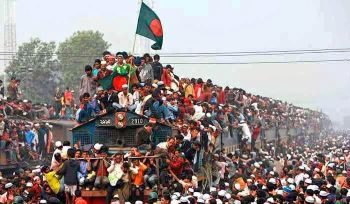
\includegraphics[]{images/pb 1.jpg}
\subsection{Agricultural crisis}
Crop agriculture in Bangladesh is, however, constrained by a number of
challenges every year. Major challenges include 1) Loss of Arable Land, 2)
Population Growth, 3) Climate Changes, 4-6) Inadequate Management Practices
(Fertilizer, Water, and Pests & Diseases), 7) Lack of Quality Seeds, and 8-10)
Inadequate Credit Support to Farmers, Unfair Price of Produces, and Insufficient
Investment in Research. Bangladesh has lost about l million ha of arable land
from 1983 to 1996. Virtually, no step has been taken by the government to arrest
this loss. The land use policy prepared by the government several years back has
not yet been implemented. Population growth poses another great threat to crop
productivity. Besides, crop agriculture in Bangladesh has become regularly
vulnerable to the hazards of climate change–flood, drought, salinity in particular.
In addition, poor management practices, especially those of pests and diseases,
fertilizer, water and irrigation have largely contributed to significant decline in
crop productivity. Small and marginal farmers that constitute majority of farm
population are constrained by poor financial resources and cannot, therefore,
afford high management costs of high input technology.
Major objective of this review article is to discuss the challenges of crop
agriculture of Bangladesh and suggest possible opportunities to address the issue
that may assist the policy makers to develop policy guidelines. 
\subsection{Electricity and fuel shortages}

Abrupt fall in gas supply from the country’s largest producing Bibiyana gas field ensued countrywide natural gas crisis affecting gas-guzzling industries, power plants, and household consumers.
Household consumers across the country have struggled in making iftar items as gas pressure fell sharply due to the gas crisis, it has been alleged.
Natural gas output from US’s oil and gas major Chevron operated Bibiyana gas field dropped by around one-third to around 800 million cubic feet per day (mmcfd) Sunday from around 1,275 mmcfd of Friday, said sources.

“Two process trains in Bibiyana gas plant are down due to maintenance since 1:15 am Sunday, which has resulted in lower production of gas from the field,” Chevron’s communications manager Shaikh Jahidur Rahman said.

“Our field operations team is working to bring the trains back online. At this moment we are unable to inform about the time required to resume full production from the field,” he said.

Energy and Mineral Resources Division (EMRD) and Power Division under the Ministry of Power, Energy and Mineral Resources (MPEMR) expressed sorrow to the consumers due to the natural gas and electricity crisis.

They hoped that the problem will be resolved soon.
%\lipsum[2]

\subsection{Education Sector}
Bangladesh is the 7th largest country in the world in population. Excluding city states like Singapore, it would make it to the top of the list in population density. The country may have already reduced its population growth, but this reduction is not nearly enough to avoid dire consequences. Currently, the country adds about 3 million to its population every year. At the same time it faces the prospect of losing land due to climate change. The world food supply is believed to be seriously affected by the climate change, which will also have a significant impact on Bangladesh. So, in order to bring stability and maintain social order by reducing the level of poverty, the country must further limit its unwanted population growth, especially among the underprivileged. However, Bangladesh may not achieve such a goal all by itself. The international community has enormous obligations to help Bangladesh achieve its objectives.
%\lipsum[3]

\subsection{Health}
Bangladesh, with a population of 1.55 million in 2012, is
one of the most densely populated countries in the world,
having a population density of 1050 per km2
.
1 The male/
female ratio is 104.9/100 and the annual population
growth rate is 1.37%.2 The population of Bangladesh is
very young as depicted by its wide-based population
pyramid. A large cohort of the young population will
enter reproductive age in the coming decades, a
phenomenon partly explaining why the adolescent (15–19
years) fertility rate in Bangladesh of 118 per 1000 women
and increasing life expectancy at birth of 69 years in
2011.3
Bangladesh Demographic and Health Survey is not
expected to decrease significantly for decades. As in other
countries, the population is ageing over time due to
decreasing fertility rates (6.3 births per woman in 1975 to
2.3 in 2011).3 consuming arsenic contaminated drinking water is
estimated at 20 million, the number of exposed persons
may well be lower because of ongoing awarenessraising activities.1,7 The challenge is to ensure access to
safe water for 100% of the population. Basic sanitation
coverage is 55% against the target of 70% by 2015.6
Although more than 90 million people in Bangladesh
shifted to fixed-point defecation in the last five years,
diarrheal diseases remain a leading cause of child and
infant morbidity. A research study shows that only 1%
of the population wash their hands with soap and water
before having a meal, 0.7% before feeding children, and
30% after defecation.8
Behavior change through hygiene promotion is a
priority to achieve the health benefit of sanitation coverage. The issue of total sanitation coverage also demands
a concept that goes beyond excreta disposal to include
the environmental sanitation issues associated with the
safe management of solid waste, household wastewater
and storm water. Waste management, including clinical
waste, solid waste, domestic and industrial wastewater,
is putting substantial burden on the environment and
creating public health risks.8 Management of clinical
waste including sharps in facilities and elsewhere is a
challenge that has to be immediately addressed.
Environmental pressures, exacerbated by climate
change, remain significant and could easily worsen if
remedial actions at the local and global levels are not
taken. While the population is expected to stabilize at
around 200 million, growing wealth and mass
population movements will place further enormous
strains on ecosystems and the living environment.1
The major communicable diseases in Bangladesh are
vaccine-preventable diseases (VPD), tuberculosis,
malaria HIV/AIDS and neglected tropical diseases
(Leprosy, Kala-azar, Lymphatic filariasis and dengue).
However the disease burden in Bangladesh has shifted
from communicable to non-communicable diseases
(NCDs) like cardiovascular diseases, diabetes, cancer,
and chronic respiratory diseases. More than half of
hospital deaths are due to NCDs. Data from the Matlab
demographic survey site showed an increasing trend of
NCD deaths from 1986 to 2006 especially due to
cardiovascular diseases.9 The study was aimed to find
out the major public health issues and challenges in
Bangladesh.
Materials and Unsafe food remains a major threat to public health4
each
year, citizens suffer from the acute effects of food
contaminated by microbial pathogens, chemical
substances and toxins. There is a need to minimize the
consumer’s exposure to unhygienic, contaminated and
adulterated food and drinks through strict laws to control
marketing of such products.1
One such factor is violence against women. This is a
widespread social problem that causes mental stress,
physical suffering and even death, and is believed to be grossly underreported. One study reveals that in
Bangladesh about 52% of men in both urban and rural
sites reported ever physically assaulting female intimate partners.5 According to the Joint Monitoring
Programme (JMP) of the World Health Organization
(WHO) and the United Nations Children’s Fund
(UNICEF), 83% of the population have access to safe
water for drinking.6 While the population at risk of consuming arsenic contaminated drinking water is
estimated at 20 million, the number of exposed persons
may well be lower because of ongoing awarenessraising activities.1,7 The challenge is to ensure access to
safe water for 100% of the population. Basic sanitation
coverage is 55% against the target of 70% by 2015.6
Although more than 90 million people in Bangladesh
shifted to fixed-point defecation in the last five years,
diarrheal diseases remain a leading cause of child and
infant morbidity. A research study shows that only 1%
of the population wash their hands with soap and water
before having a meal, 0.7% before feeding children, and
30% after defecation.8
Behavior change through hygiene promotion is a
priority to achieve the health benefit of sanitation coverage. The issue of total sanitation coverage also demands
a concept that goes beyond excreta disposal to include
the environmental sanitation issues associated with the
safe management of solid waste, household wastewater
and storm water. Waste management, including clinical
waste, solid waste, domestic and industrial wastewater,
is putting substantial burden on the environment and
creating public health risks.8 Management of clinical
waste including sharps in facilities and elsewhere is a
challenge that has to be immediately addressed.
Environmental pressures, exacerbated by climate
change, remain significant and could easily worsen if
remedial actions at the local and global levels are not
taken. While the population is expected to stabilize at
around 200 million, growing wealth and mass
population movements will place further enormous
strains on ecosystems and the living environment.1
The major communicable diseases in Bangladesh are
vaccine-preventable diseases (VPD), tuberculosis,
malaria HIV/AIDS and neglected tropical diseases
(Leprosy, Kala-azar, Lymphatic filariasis and dengue).
However the disease burden in Bangladesh has shifted
from communicable to non-communicable diseases
(NCDs) like cardiovascular diseases, diabetes, cancer,
and chronic respiratory diseases. More than half of
hospital deaths are due to NCDs. Data from the Matlab
demographic survey site showed an increasing trend of
NCD deaths from 1986 to 2006 especially due to
cardiovascular diseases.9 The study was aimed to find
out the major public health issues and challenges in
Bangladesh.
Materials and
%\lipsum[4

% \section{Government responses}
% \subsection{Monetary Policy}
% \subsection{Fiscal Policy}
% \section{Gradually Fall Of A Country}
% \subsection{Foreign Loan}
% \subsection{Crashed GDP}

% {\bf Paper I.} \lipsum[75]

% {\bf Paper II.} \lipsum[75]

% {\bf Paper III.} \lipsum[75]

% {\bf Paper IV.} \lipsum[75]

% \section{Conclusions}
% \lipsum[5]

\newpage


\printbibliography[heading=bibintoc, title={References}]

\end{document}
